% demosaicado_bilineal_tikz.tex
% Gráfica TikZ del proceso de demosaicado bilineal - Versión corregida con superposición de esquinas

\begin{figure}[h]
\centering
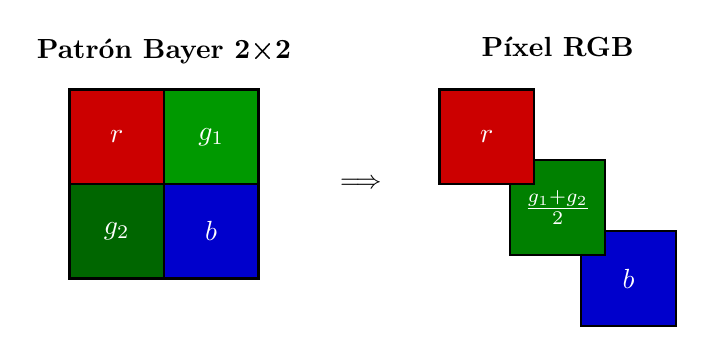
\begin{tikzpicture}[
    font=\small,
    pixel/.style={rectangle, draw=black, minimum width=1.2cm, minimum height=1.2cm, inner sep=0}
]

% ============================================
% PATRÓN BAYER ORIGINAL (2x2 RGGB)
% ============================================

% Cuadrante superior izquierdo (rojo)
\fill[red!80!black] (-1.2,0) rectangle (0,1.2);
\draw[black, thick] (-1.2,0) rectangle (0,1.2);
\node[white, font=\bfseries] at (-0.6,0.6) (r) {$r$};

% Cuadrante superior derecho (verde 1)
\fill[green!60!black] (0,0) rectangle (1.2,1.2);
\draw[black, thick] (0,0) rectangle (1.2,1.2);
\node[white, font=\bfseries] at (0.6,0.6) (g1) {$g_1$};

% Cuadrante inferior izquierdo (verde 2)
\fill[green!40!black] (-1.2,-1.2) rectangle (0,0);
\draw[black, thick] (-1.2,-1.2) rectangle (0,0);
\node[white, font=\bfseries] at (-0.6,-0.6) (g2) {$g_2$};

% Cuadrante inferior derecho (azul)
\fill[blue!80!black] (0,-1.2) rectangle (1.2,0);
\draw[black, thick] (0,-1.2) rectangle (1.2,0);
\node[white, font=\bfseries] at (0.6,-0.6) (b) {$b$};

% Marco exterior del patrón
\draw[black, very thick] (-1.2,-1.2) rectangle (1.2,1.2);

% Título
\node[above, align=center, font=\bfseries] at (0,1.4) 
    {Patrón Bayer 2×2};

% ============================================
% FLECHA DE PROCESO
% ============================================
\node at (2.5,0) {$\Longrightarrow$};

% ============================================
% PÍXEL RESULTANTE (CARTAS SUPERPUESTAS CON ESQUINAS)
% ============================================

% Parámetros
\def\cardsize{1.2cm}
\def\overlap{0.3cm} % L/4 = 1.2cm/4 = 0.3cm
\def\shift{0.9cm} % cardsize - overlap = 1.2 - 0.3 = 0.9cm
\def\sqareorigin{3.5cm}

% ORDEN: Primero dibujamos la de atrás (B), luego la del medio (G), luego la del frente (R)

% Azul (B) - atrás - más desplazada hacia abajo y derecha
\fill[blue!80!black]                (\sqareorigin+2*\shift            , -2*\shift) rectangle (\sqareorigin+2*\shift+\cardsize, -2*\shift+\cardsize);
\draw[black, thick]                 (\sqareorigin+2*\shift            , -2*\shift) rectangle (\sqareorigin+2*\shift+\cardsize, -2*\shift+\cardsize);
\node[white, font=\bfseries] at     (\sqareorigin+2*\shift+\cardsize/2, -2*\shift+\cardsize/2) (B) {$b$};

% Verde (G) - medio - desplazada un shift
\fill[green!50!black]               (\sqareorigin+\shift              , -  \shift) rectangle (\sqareorigin+\shift+\cardsize, -\shift+\cardsize);
\draw[black, thick]                 (\sqareorigin+\shift              , -  \shift) rectangle (\sqareorigin+\shift+\cardsize, -\shift+\cardsize);
\node[white, font=\bfseries] at     (\sqareorigin+\shift+\cardsize/2  , -  \shift+\cardsize/2) (G) {$\frac{g_1 + g_2}{2}$};

% Rojo (R) - frente - posición base (sin desplazar)
\fill[red!80!black]                 (\sqareorigin,0) rectangle (\sqareorigin+\cardsize           , \cardsize);
\draw[black, thick]                 (\sqareorigin,0) rectangle (\sqareorigin+\cardsize           , \cardsize);
\node[white, font=\bfseries] at     (\sqareorigin+\cardsize/2         , \cardsize/2) (R) {$r$};

% Título del píxel resultante
\node[above, font=\bfseries] at (\sqareorigin+\cardsize/2+\shift, 1.5) {Píxel RGB};

\end{tikzpicture}
\caption{Proceso de demosaicado bilineal para patrón Bayer RGGB. Los canales de color se superponen para formar el píxel RGB final.}
\label{fig:demosaicado_bilineal}
\end{figure}
